\documentclass{article}
\usepackage[utf8]{inputenc}
\usepackage{hyperref}
\usepackage{tikz}
\usepackage{pifont}
\usepackage{natbib}
\bibliographystyle{unsrtnat}
\graphicspath{{/home/feideu/Work/Gnunet/schemafuzz/docs/}}
\usepackage{graphicx}
\usepackage{pdfpages}
\usepackage{url}
\usepackage{emp}
\usepackage{subcaption}
\usetikzlibrary{shapes.arrows,chains}
\usepackage[english]{babel}
\newcommand\tab[1][1cm]{\hspace*{#1}}
% Definition of \maketitle
\makeatletter         
\def\@maketitle{

\begin{figure}[!h]
\centering
\begin{minipage}{0.6\textwidth}
  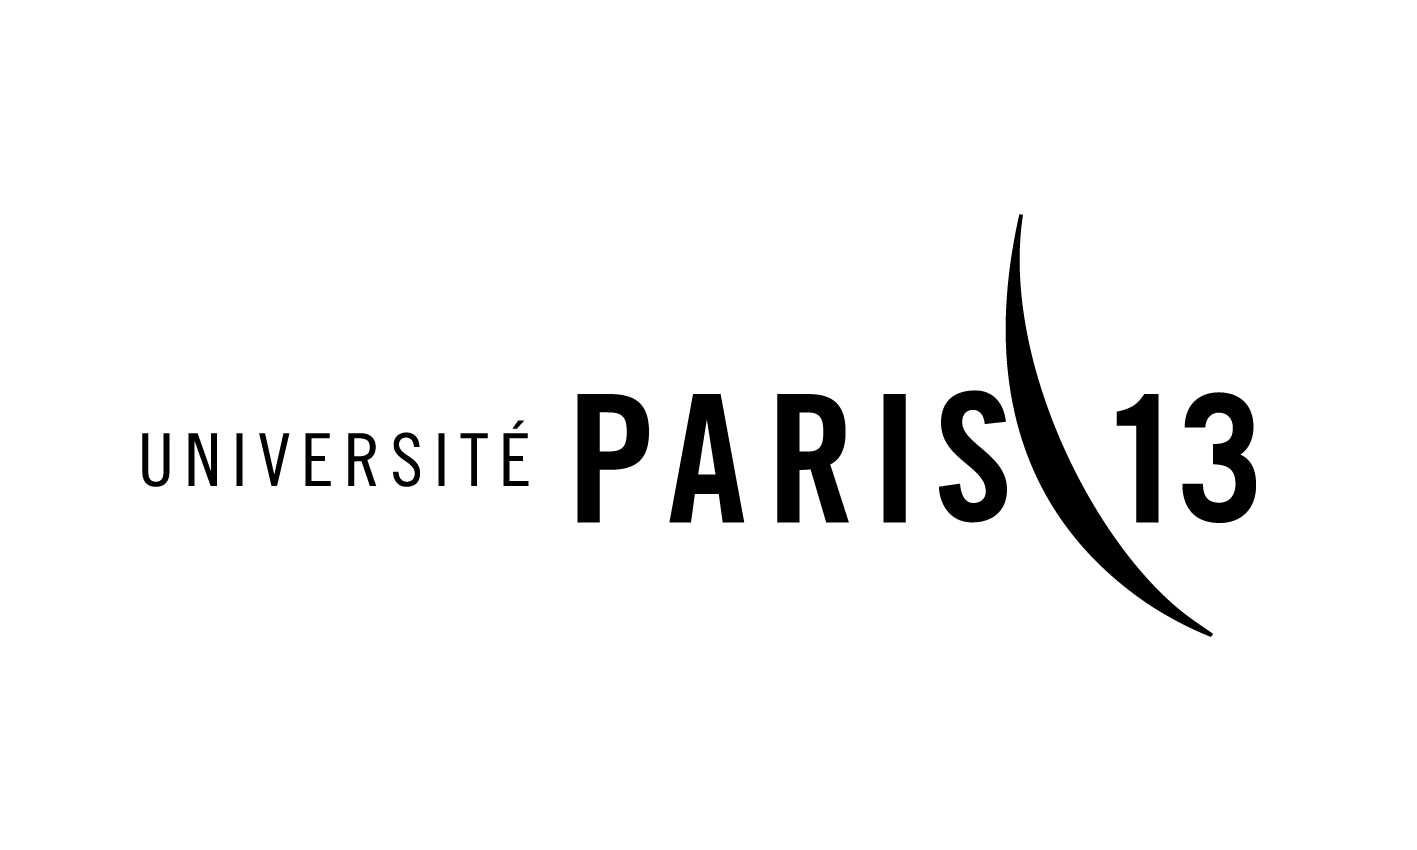
\includegraphics[width=1\linewidth]{LogoP13.png}
\end{minipage}%
\begin{minipage}{0.6\textwidth}
  
\includegraphics[width=1\linewidth]{LogoBFH.jpeg}
\end{minipage}
\end{figure}

\vspace*{\fill}
\begin{center}
{\Huge \bfseries \sffamily \@title }\\[4ex] 
{\Large  \@author}\\[4ex] 
\@date\\[8ex]
\end{center}}
\makeatother

\title{Database Oriented Fuzz Testing Tool Development}
\author{Ulrich "Feideus" Erwan}

\begin{document}
\begin{empfile}

\maketitle

\vspace*{\fill}
\underline{Supervisors}: Christian Grothoff, Pierre Boudes 	\\*
\tab[0.4cm] \underline{Promotion}: 2017-2018
\clearpage

\tableofcontents
\clearpage

	\abstract
The concept of fuzz testing is the result of submitting unexpected data to a software. It is used in software development in order to reveal errors or approximations in the source code of a project. Several approaches exist in order to pursue this goal such as focusing a specific type of data or using concepts that subscribe in the field of machine learning. This project is an implementation of the fuzz testing strategy focusing on the management of a database's content.  \\*
The purpose of this documentation is to provide an introduction on the concept of fuzz testing and to describe precisely an example of implementation. \\*
It is hoped that it will give more insights on the philosophy and the drive that motivated this work as well as a description of the design of the SchemaFuzz tool for its users and contributers.

\bigskip

Le concept du Fuzz testing est le resultat de la soumission de données inapropriées à un programme cible. Ce concept est utilisé au cours du developement dans le but de reveler les erreurs d'implementation ainsi que les failles de securité dans le code source d'un projet informatique. Plusieurs approches differentes peuvent permettrent d'atteindre ce but telles que la concentration sur un type particuler de données ou encore l'utilisation de concepts externes comme l'apprentissage machine. Ce projet est une implementation de la strategie du fuzz testing en se concentrant sur la gestion d'objets issues d'une base de données \\*
Le but de cette documentation est de fournir une introduction au concept du fuzz testing et de decrire précisement un exemple d'implémentation. \\*
Nous nourissons l'espoir qu'elle apportera de plus amples détails sur la philisophie et sur les motivation qui soutiennent ce projet ainsi que sur le désign de l'outil SchemaFuzz pour ses utilisateurs et contributeurs. 

	
	\section{Introduction} 
	
This project is meant to provide an secure development tool that uses a database oriented "fuzzing" strategy.  
Where a traditional fuzzer would send malformed input to a program, SchemaFuzz modifies the content of a database to test that program's behavior when stumbling on  unexpected data. \\*
This tool's objective is to bring up the bugs and security breaches that the code may contain regarding the retrieving and usage  of a database's content by stressing it with corrupted data.
This tool is still at an alpha state; its development will is still in progress and will be the subject of further publications which will lead to updates in this document. 
	\clearpage

	
	\section{Context and Perimeter} 
		\subsection{Context}

SchemaFuzz uses the principle of "fuzz testing" or "fuzzing" to help find out which are the weak code paths of one's project. It is usually defined as: 

\begin{quotation} "an automated software testing technique that involves providing invalid, unexpected, or random data as inputs to a computer program". \end{quotation}\cite{fuzzing}		
	
This quote is well illustrated by the following example :
				\begin{quotation}
Lets consider an integer in a program, which stores the result of a user's choice between 3 questions. When the user picks one, the choice will be 0, 1 or 2. Which makes three practical cases. But what if we transmit 3, or 255? We can, because integers are stored in a static size variable. If the default case hasn't been implemented securely, the program may crash and lead to any kind of security issue such as: (un)exploitable buffer overflows, DoS, ... 
				\end{quotation}

Fuzz testing has been used since the 90's to test one's software robustness.
The first generation of fuzzing tools was composed of primitive input injections which was described with the "infinite monkey theorem" analogy.
It is divided in severals categories that each focus on a specific type of input.
 
UI fuzzing focuses on button sequences and more generically any kind of user input during the execution of a program. This principle has already been successfully used in existing fuzzing tools such as  "MonkeyFuzz".

Certificate fuzzing is another interesting fuzzing approach that has emerged especially after it was introduced by \cite{Certif} in $Development$ $of$ $Intelligent$ $Digital$ $Certificate$ $Fuzzer$ $Tool$

However, SchemaFuzz is a database oriented fuzzer. This means that it focuses on triggering unexpected behavior related to the usage of a external database content   

This tool is meant to help developers, maintainers and more generically anyone that makes use of data coming from a database under his influence in their task. A good way to sum up the effect of this tool is to compare it with an "cyber attack simulator".
This means that the idea behind it is to emulate the damage that an attacker may cause subtly or not to a database he possesses privileges on. This might in theory go from a simple boolean flip (subtle modifications) to removing/adding content to purely and simply destroying or erasing all the content of the database.
SchemaFuzz focuses on the first part: modification of the content of the database by sequential modifications that may or may not overlap. These modifications may be   aggressive or subtle.
It is interesting to point out that this last point also qualifies SchemaFuzz as a good "database structural flaw detector".
That is to say that errors typically triggered by a poor management of a database (wrong data type usage, incoherence between database structure and use of the content etc ...) might also appear clearly during the execution.
For a more in depth description of different fuzzing approaches, one can refer to $A$ $systematic$ $review$ $of$ $fuzzing$ $techniques$ \cite{Systematic}

		\subsection{Perimeter}
This tool implements some of the SchemaSpy tool's source code. More precisely, it uses the portion of the code that detects and stores the target database's structure as well the data type for each of the fields that it contains. This project's design revolves around the adaptation of this existing code. Developing the functionalities required to test the usage of the database content by any kind of utility is the main stake of SchemaFuzz.  		
The resulting software will generate a group of human readable reports on each modification that was performed.		
		\begin{figure} [h!]
		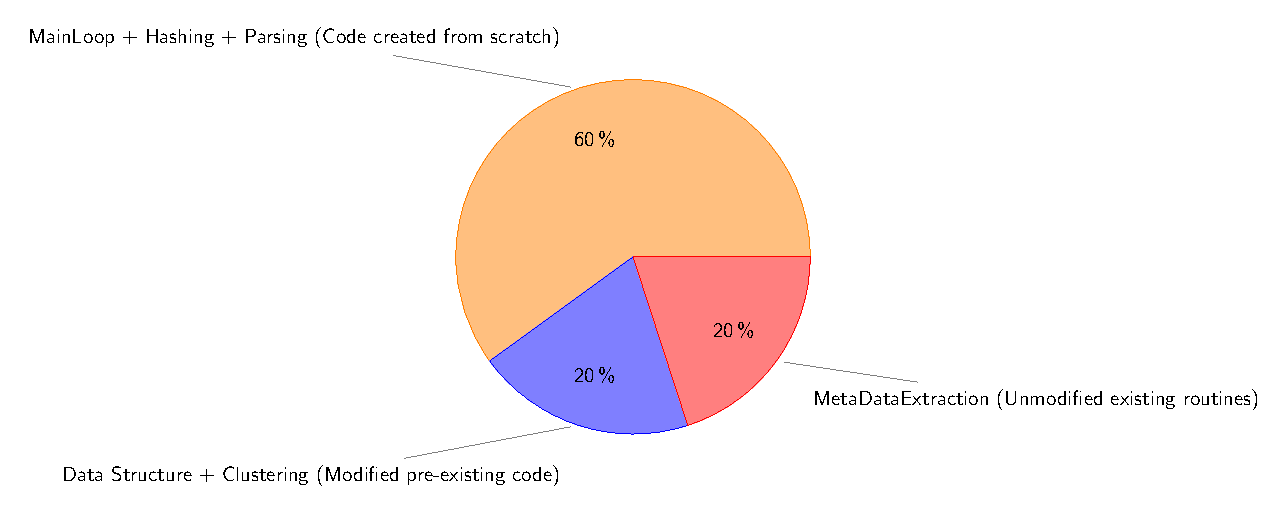
\includegraphics[width=\textwidth]{codeOriginDiagram.pdf}
		\caption{Shows the nature of the code for every component. The slice size is a rough estimation.}
		\end{figure}
		\subsection{When to use it}
SchemaFuzz is a useful tool for developers trying secure a piece of software that uses database resources. In its current state, Schemafuzz is only compatible with C language and more specifically with GDB compatible softwares. The DBMS (which is the SQL interpretor used by the target software) has to grant access to the target database through credentials passed as argument to this tool.

Since this tool does not have a rollback feature yet to restore the first state of the target database, the database being fuzzed will end up in a randomly modified state that may not be suitable for production. Thus, it is strongly advised to use a copy of the target database rather than the production material
		\clearpage

	\section{Design}
		\subsection{Generic explanation}
The code for the core of the program is organized as follows:
		\begin{itemize}
		\item{Mutation/data-set used as a way to store the inputs, outputs and other interesting data from the modification that was performed on the target database}
		\item{The mutation tree, used to store the mutations coherently}
		\item{An analyzer that scores the mutations to influence the paths that will be explored afterwards}
		\end{itemize}
This organization will be detailed and discussed in the following sections.

\begin{figure} [h!]
\includegraphics[scale=0.7]{StructuralDiagram.pdf}
\caption{Structural organization of the different components}
\end{figure}

		 \clearpage
\begin{figure} [h!]
\centering

\includepdf[pages={2},scale=0.85]{EndToEndDiagram.pdf}
\caption{Main Loop work flow chart}
\end{figure}
		 \clearpage		 
		 
		 
		 
		\subsection{SchemaSpy legacy/meta data extraction}
The only job of the meta data extraction routine is to initialize the connection to the database and retrieve its meta data at the   beginning of the execution (before any actual SchemaFuzz code is run). These meta data include data types, table and table column names, views and foreign/primary key constraints. Having this pool of meta data in a Java object shape allows the main program to properly mark off what the possibilities are in terms of modifications as well as dealing with the possible constraints on the different tables. The modifications that will be created during the main loop will be designed to respect the data type constraints built from the result of this extraction. 

\begin{figure} [h!]
\centering
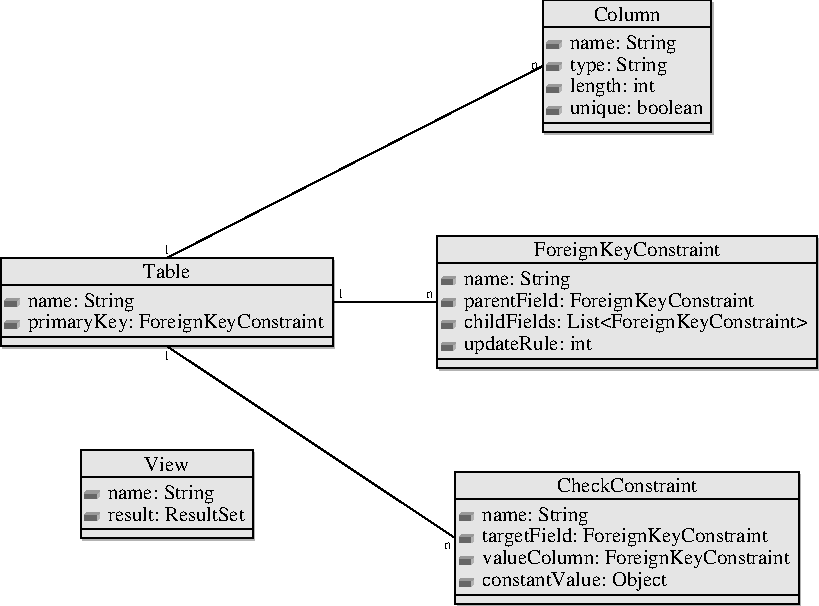
\includegraphics[width=\textwidth]{MetaDataExtractionDiagram-1.pdf}
\caption{Objects returned by the meta data extraction routine.}
\end{figure}

In order to do that, the user shall provide this set of mandatory database related arguments
			\begin{itemize}
 				\item The driver to the corresponding database DBMS (only support Postgre at the moment)
 				\item The credentials to be used to access the database.
 				\item The name of the database
			\end{itemize}
		\subsection{SchemaFuzz Core}		
			\subsubsection{Constraints}
The target database often contains constraints on one or several tables. These constraints have to be taken into account in the process of fabricating mutations as most of the time they restrict the possible values that the pointed field can take. These restrictions can take the shape of a \underline {Not Null} constraint, \underline{Check} constraint, \underline{Foreign key} constraint (value has to exist in some other table's field) or \underline{Primary key} constraint (no doublets of value allowed). These constraints are stored as Java objects instantiated from the corresponding class.
\bigskip

\begin{figure} [h!]
\centering
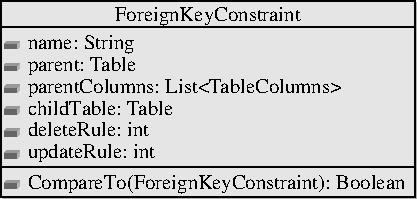
\includegraphics[width=\textwidth]{ForeignKeyClassDiagram-1.pdf}
\caption{Class diagram of the ForeignKeyConstraint Java object}
\end{figure}

\bigskip

The last two ones are the problematic ones. They imply specific work before applying any mutations to make sure that the value respect all the restrictions. before doing anything else after the meta data extraction is done, SchemaFuzz performs an update of all the existing constraints on the database to add the CASCADE clause. This allows the values bonded by a foreign key constraints to take effect. The tool reverts these updates to take the constraints back to their initial state before the program exits.
				\paragraph{Primary key constraints (PKC):}
The primary key constraints require an extra DB query that checks the existence of the value in the column. If the value already exists (the query's result is not empty), the mutation will be dropped before being executed.
				\paragraph{Foreign key constraints (FKC):}
The foreign Key constraint is the trickiest one. Its inherent nature bonds two values of different table columns where the value being referenced is called the father, and the referencing field, the child. In order to change one of the two values, the other has to be changed accordingly in the same transaction. SchemaFuzz uses the semantics of the CASCADE clause to make the change possible. This clause allows the DBMS to automatically change the value of the child if the father has been changed.
This mechanic allows to change any of the bounded values by changing the father's value.
To do so, the software has a way to transfer the mutation from a child to its parent.

  				
			\subsubsection{Mutations}
A mutation is a Java object that bundles all the informations that are used to perform a modification in the database. Every mutation is linked to its parent and inherits some of his parent's data. In the case of a follow up mutation the child inherits the database row that was his parent's target. Therefore the initial state (state before the injection of the modification) of its target is exactly the final state (state after injection of the modification) of his parent's target. A mutation is created for each iteration of the main loop and represents a single step in the progress of the fuzzing.
It also holds the information concerning the result of the injection in the shape of a data vector. This data vector is then used to perform a clustering calculus to determine the "uniqueness" of the mutation. This value is also stored inside the mutation object and is used as the weight of this mutation in the tree.

\bigskip

\begin{figure} [h!]
\centering
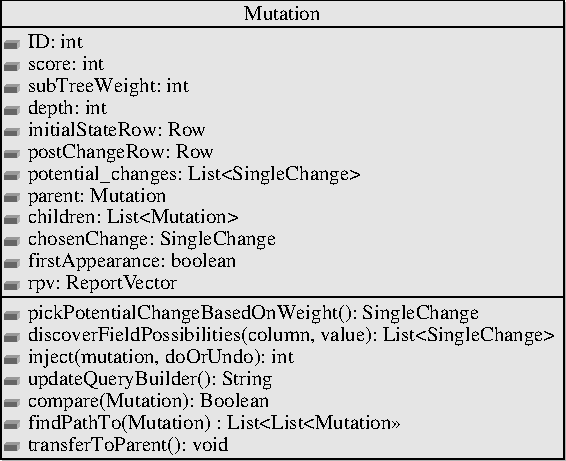
\includegraphics[scale=0.9]{MutationClassDiagram-1.pdf}
\caption{Structure of a Mutation}
\end{figure}

\clearpage
				
A branch is a succession of mutation that share the same database row as their modification target.
The heuristics determining the next mutation's modification are still primitive and will be thinly adjusted in futures versions.								 
				\paragraph{Creating malformed data} 
As the goal of running SchemaFuzz is to submit unexpected or invalid data to the target software, it is necessary to understand that fuzzing a complex type such a timestamps variables has nothing to do with fuzzing a trivial boolean. In practice, a significant part of this matter could absolutely be the subject of a more abstract work. We focused here on a simple approach (as a first step).
After retrieving the current row being fuzzed (may it be a new row or a previously fuzzed row), the main loop explores the different modification possibilities.
The main loop then builds the possible modification for each of the fields for the current row. The possible modifications that this tool can produce at the moment are : \\ % add complete list of the modifications that CAN be gener$ 
				Boolean types:
				\begin{itemize}						
					\item Swapping the existing value (F $\mapsto$ T OR T $\mapsto$ F)
				\end{itemize}
				Integer types:
				\begin{itemize}
		
					\item Extreme values ($0, \texttt{MAXVALUE}$ etc.)
					\item Random value ($0<\texttt{value}<\texttt{MAXVALUE}$ etc.)
					\item Increment/Decrement the existing value ($332 \mapsto 333$ OR $332 \mapsto 331$)
				\end{itemize}
				String types:
				\begin{itemize}
					\item Change string to ``aaa" (``Mount Everest" $\mapsto$ ``aaa")
					\item Increment/Decrement ASCII character at a random position in the string (``Mount Everest" $\mapsto$ ``Mount Fverest")
				\end{itemize}
					Date Types: (implemented but not fully functional)			
				\begin{itemize}
					\item Increment/Decrement date by 1 day/minutes depending on the precision of the date
					\item Set date to $01/01/1970$ 
				\end{itemize}
These "abnormal" values might in fact be totally legit in some cases. In that case the analyzer will rank the mutation rather poorly, which will lead to this tree path not being likely to be developed further.
				\\*
				\paragraph{SQL handling}
All the SQL statements are generated within the code. This means that the data concerning the current and future state of the mutations have to be   precise. Otherwise, the SQL statement is   likely to fail. Sadly, since SchemaFuzz only supports PostgreSQL, the implemented syntax follow the one of Postgre
DBMS. The statement is built to target the row as precisely as possible, meaning that it uses all of the non fuzzed values from the row to avoid updating other row accidentally. Only the types that can possibly be fuzzed will be used in the building of the SQL statement. Since this part of the code is delicate in the sense that it highly depends on an arbitrary large pool of variables from various types it is has a tendency of crashing. 
				
				\paragraph{Injecting:}
The injection process sends the built statement to the DBMS so that the modification can be operated. After the execution of the query, depending of the output of the injection (one modification, several modifications, transfer) informations are updated so that they can match the database state after the modification. If the modification failed, no trace of this mutation is kept, it is erased and the execution goes on like nothing happened.  				
				\paragraph{Special case (mutationTransfer):}
The mutation transfer is a special case of a modification being applied to the database.
It is triggered when the value that was supposed to be fuzzed is under the influence of a FKC as the child.
In the case a FKC (in CASCADE mode), only the father can be changed, which also triggers the same modification on all of his children. The algorithm then "transfers" the modification from the original mutation to its father.
After injecting the transfered mutation, the children mutation is modified but the modification cascades on some parts of the database that was not meant to be changed.
Hopefully, this does not impact the life of the algorithm until this mutation is reverted (see next paragraph).
				\paragraph{Do/Undo routine:}
The Do/Undo mechanism is at the center of this software. Its behavior is crucial for the execution and will have a strong impact on the coherence of the data nested in the code or inside the target database throughout the runtime.
This mechanism allows the algorithm to revert a previous mutation or, if necessary inject it one more time. 
Undoing a mutation applies the exact opposite modification that was originally applied to the database ending up in recovering the same database state as before the mutation was injected.
Reverting mutations is the key to flawlessly shifting the current position in the mutation tree.
The case of the transfered mutation is no exception to this. In this case, the mutation applied changes on an unknown number of fields in the database. But, the FKC still bounds all the children to their father at this point (this is always the case unless this software is not used as intended).  
Changing the father's field value back to its original state will propagate the original values back on all the children.
This mechanism might trigger failing mutations in some cases (usually mutations following a transfer). This issue will be addressed in the known issues section. 

				\subsubsection{Choosing pattern}
For each iteration of the main loop, a modification has to be picked up as the next step in the fuzzing process. This is done by considering the current state of the tree. Three parallel code paths can be triggered from this point.
				\begin{itemize}
				\item{Continue on the current branch of the tree (triggered if the last mutation scored better than its parent)}
				\item{Pick an existing branch in the tree and grow it (triggered if the last mutation scored worse than its parent on a 50/50 chance with the next bullet)}
				\item{Start a new branch (triggered if the last mutation scored worse than its parent on a 50/50 chance with the previous bullet)}
				\end{itemize}				
				
				\bigskip
			\begin{figure}[ht!]
			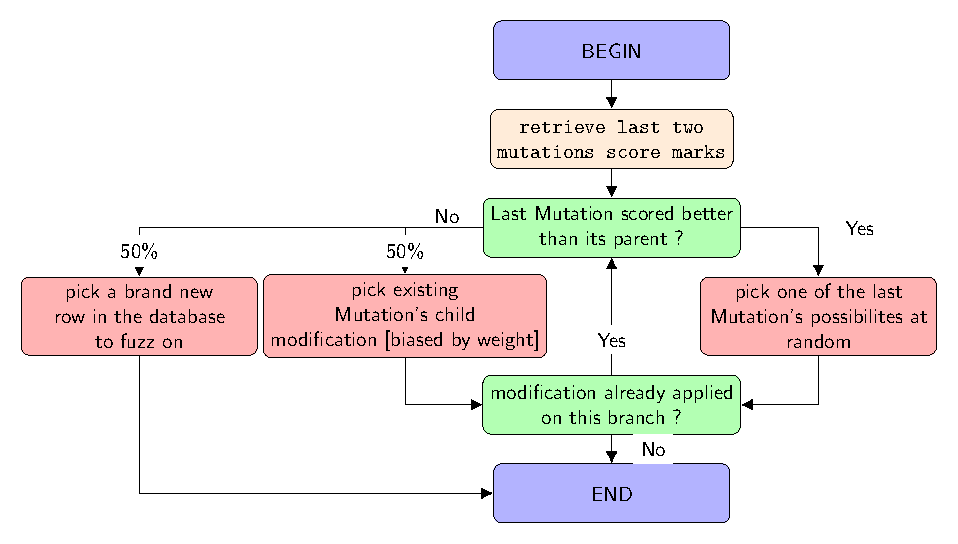
\includegraphics[width=\textwidth]{pickingPaternDiagram.pdf}
			\caption{Diagram that shows, for each iteration of the main loop, how the next modification is chosen}
			\end{figure}			
		
						\bigskip
			\subsubsection{Tree Based data structure}
All the mutations that are injected at least once in the course of the execution of this software are stored properly in a tree data structure. Having such a data structure makes parent-children relations between mutations possible. The tree follows the traditional definition of the a n-ary algorithmic tree.
It is made of nodes (mutations) including a root (first mutation to be processed on a field selected randomly in the database)  
Each node has a number of children that depends on the ranking its mutation and the number of potential modifications that it can perform.
				\paragraph{Weight}
Weighting the nodes is an important part of the runtime. Each mutation has a weight that is equal to the ranking the analyzer returns as an output. This value reflects the mutation's value. If it had an interesting impact on the target program behavior (if it triggered new bugs or uncommon code paths) than this value is high. The weight is then used as a mean of determining the upcoming modification. The chance that a mutation gets a child is directly proportional to its weight.

				\paragraph{Path}:
Since the weighting of the mutation allows to go back to previous more interesting mutations, there is a need for a path finding mechanism. In practice, this routine determines the chain of node that separates two nodes in the tree. This is done by, from both nodes, going in the direction of the root until a common ancestor is found. Fusing the lists of both chains results in creating the full path between the two nodes. The path is then used when the main loop goes through the undo mechanism. Undoing from mutation A to mutation B is implemented as undoing every mutation between A and B

\bigskip

\begin{figure}[h!] 
\centering
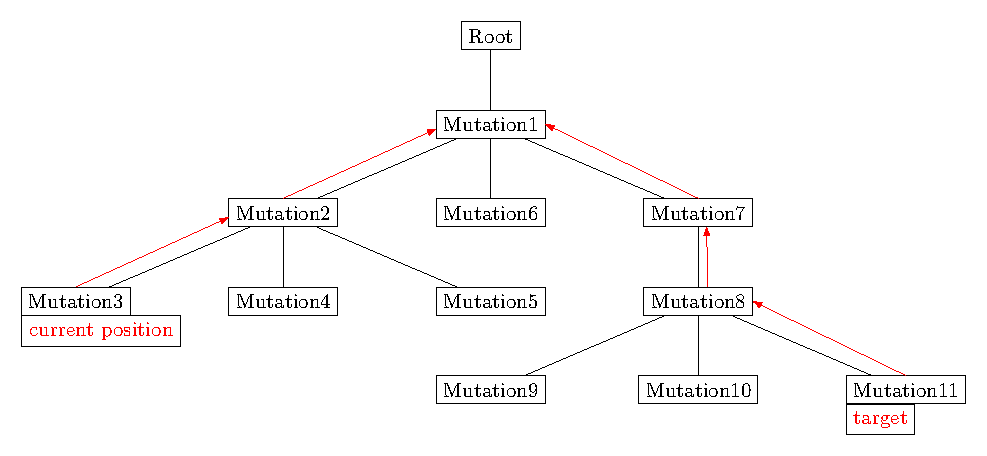
\includegraphics[width=\textwidth]{CommonAncestorDiagram.pdf}
\caption{Example of path between two nodes in the tree}
\end{figure}

\bigskip
			\subsubsection{The analyzer}
Analyzing the output of the target program is another critical part of SchemaFuzz. The analyzer parses in the stack trace of the target software's execution in order measure how interesting the output of the execution was. Since crashes and unexpected behavior from the target software is what the tool is triggering, it is the main criteria of a valuable mutation. A stack trace is a text block structured to present all the information related to a crash during a software's execution. The analyzer in its current state only observes stack traces generated from the GDB C debugger.  
				\paragraph{Stack Trace Parser}
The stack trace parser is a separate Bash script that processes stack traces generated by the GDB C language debugger and stores all the relevant informations (function's name, line number, file name) into a Java object. The parser also generates a human readable file for each mutation that synthesizes the stack trace values as well as additional interesting information useful for other mechanisms (that also require parsing). These additional informations include the path from root to mutation (useful for rolling back the database to a specific state).
				\paragraph{Hashing}
The clustering algorithm takes a triplet of numerical values as an input. Therefore, the stack trace of a mutation has to be hashed into a triplet of numerical values. This set of value is used as a representation of the original stack trace object.
Hashing is usually defined as follows : 
				\begin{quotation}
"A hash value (or simply hash), also called a message digest, is a number generated from a string of text. The hash is substantially smaller than the text itself, and is generated by a formula in such a way that it is extremely unlikely that some other text will produce the same hash value."
				\end{quotation} \cite{Hashing} \\*
				
In the present case, we used a different approach. Since proximity between two stack traces is the key to a relevant ranking, it is mandatory to have a hashing function that preserves the proximity of two strings. 
In that regard, we implemented a version of the Levenshtein Distance algorithm.
This algorithm can be explained by the following statement:
				\begin{quotation}
"The Levenshtein distance between two words is the minimum number of single-character edits (insertions, deletions or substitutions) required to change one word into the other."
				\end{quotation} \cite{LevensteinDistance}\\*		 
				
\begin{figure} [h!]
\centering
\begin{tabular}{ | l | l | l | l | l | l | c | r | }
  \hline			
  E & X & E & M & P & L & E &  \\ \hline
  \ding{51}  & \ding{51}  & \ding{56}  & \ding{51}  & \ding{51}  & \ding{51}  & \ding{51} & \ding{56}  \\\hline
  E & X & A & M & P & L & E & S \\
  \hline  
\end{tabular}
\caption{Example of the levenshtein distance concept.}
\end{figure}

The distance for this example is $2\div8\times100$				
				
After hashing the file name and the function name into numerical values trough Levenshtein distance, the analyzer creates the triplet that numerically represents the stack trace being parsed. This triplet will be used in the clustering method detailed in the following paragraph.
It is interesting to note that this triplet is not the most accurate representation of a stack trace. The analyzer will be improved in the future is that regard.

				\paragraph{The scoring mechanism}
The "score" (or rank) of a mutation is a numerical value that reflects how interesting the outcome was. Unique crashes and unexpected behavior are what makes a mutation valuable since it indicates a wrongly implemented code piece in the target source in most cases. Unique crashes detection and processing was brightly detailed in Mr \cite{Unique}'s work which I recommend consulting for further explanation. This value is calculated through a modified version of a K-means clustering method precisely detailled by \cite{Kmeans}.
This clustering mechanism runs as follows:
	\begin{itemize}
	\item{Represent the triplets in a 3 dimensional space}
	\item{Create clusters that includes most similar triplets}
	\item{Calculate the centroid of each cluster}
	\item{Calculate the Euclidean distance between the current mutation's triplet and all the centroids}
	\item{Add up all the distances generated by the last step into a single value}
	\end{itemize}

The centroid of a cluster is the triplet of values that define the mathematical center of a cluster.
the Euclidean distance is defined as
	\begin{quotation}
	In mathematics, the Euclidean distance or Euclidean metric is the "ordinary" straight-line distance between two points in Euclidean space
	\end{quotation}\cite{EuclideanDistance} \\*
	
If a triplet represents a unique crash it will be placed far away in the Euclidean space. This induces that the sum of the Euclidean distances to the centroids will be a high value compared to a common crash. This sum is then used as the "score" of the mutation. 

Mutations that do not trigger any crash result in having a null score. Therefore, the side of the tree they are in has a lower statistical chance of being chosen for further exploration.

For a more concrete view of what the analyzer outputs, please refer to the Result and Example section.

\clearpage

\begin{figure}
\centering
  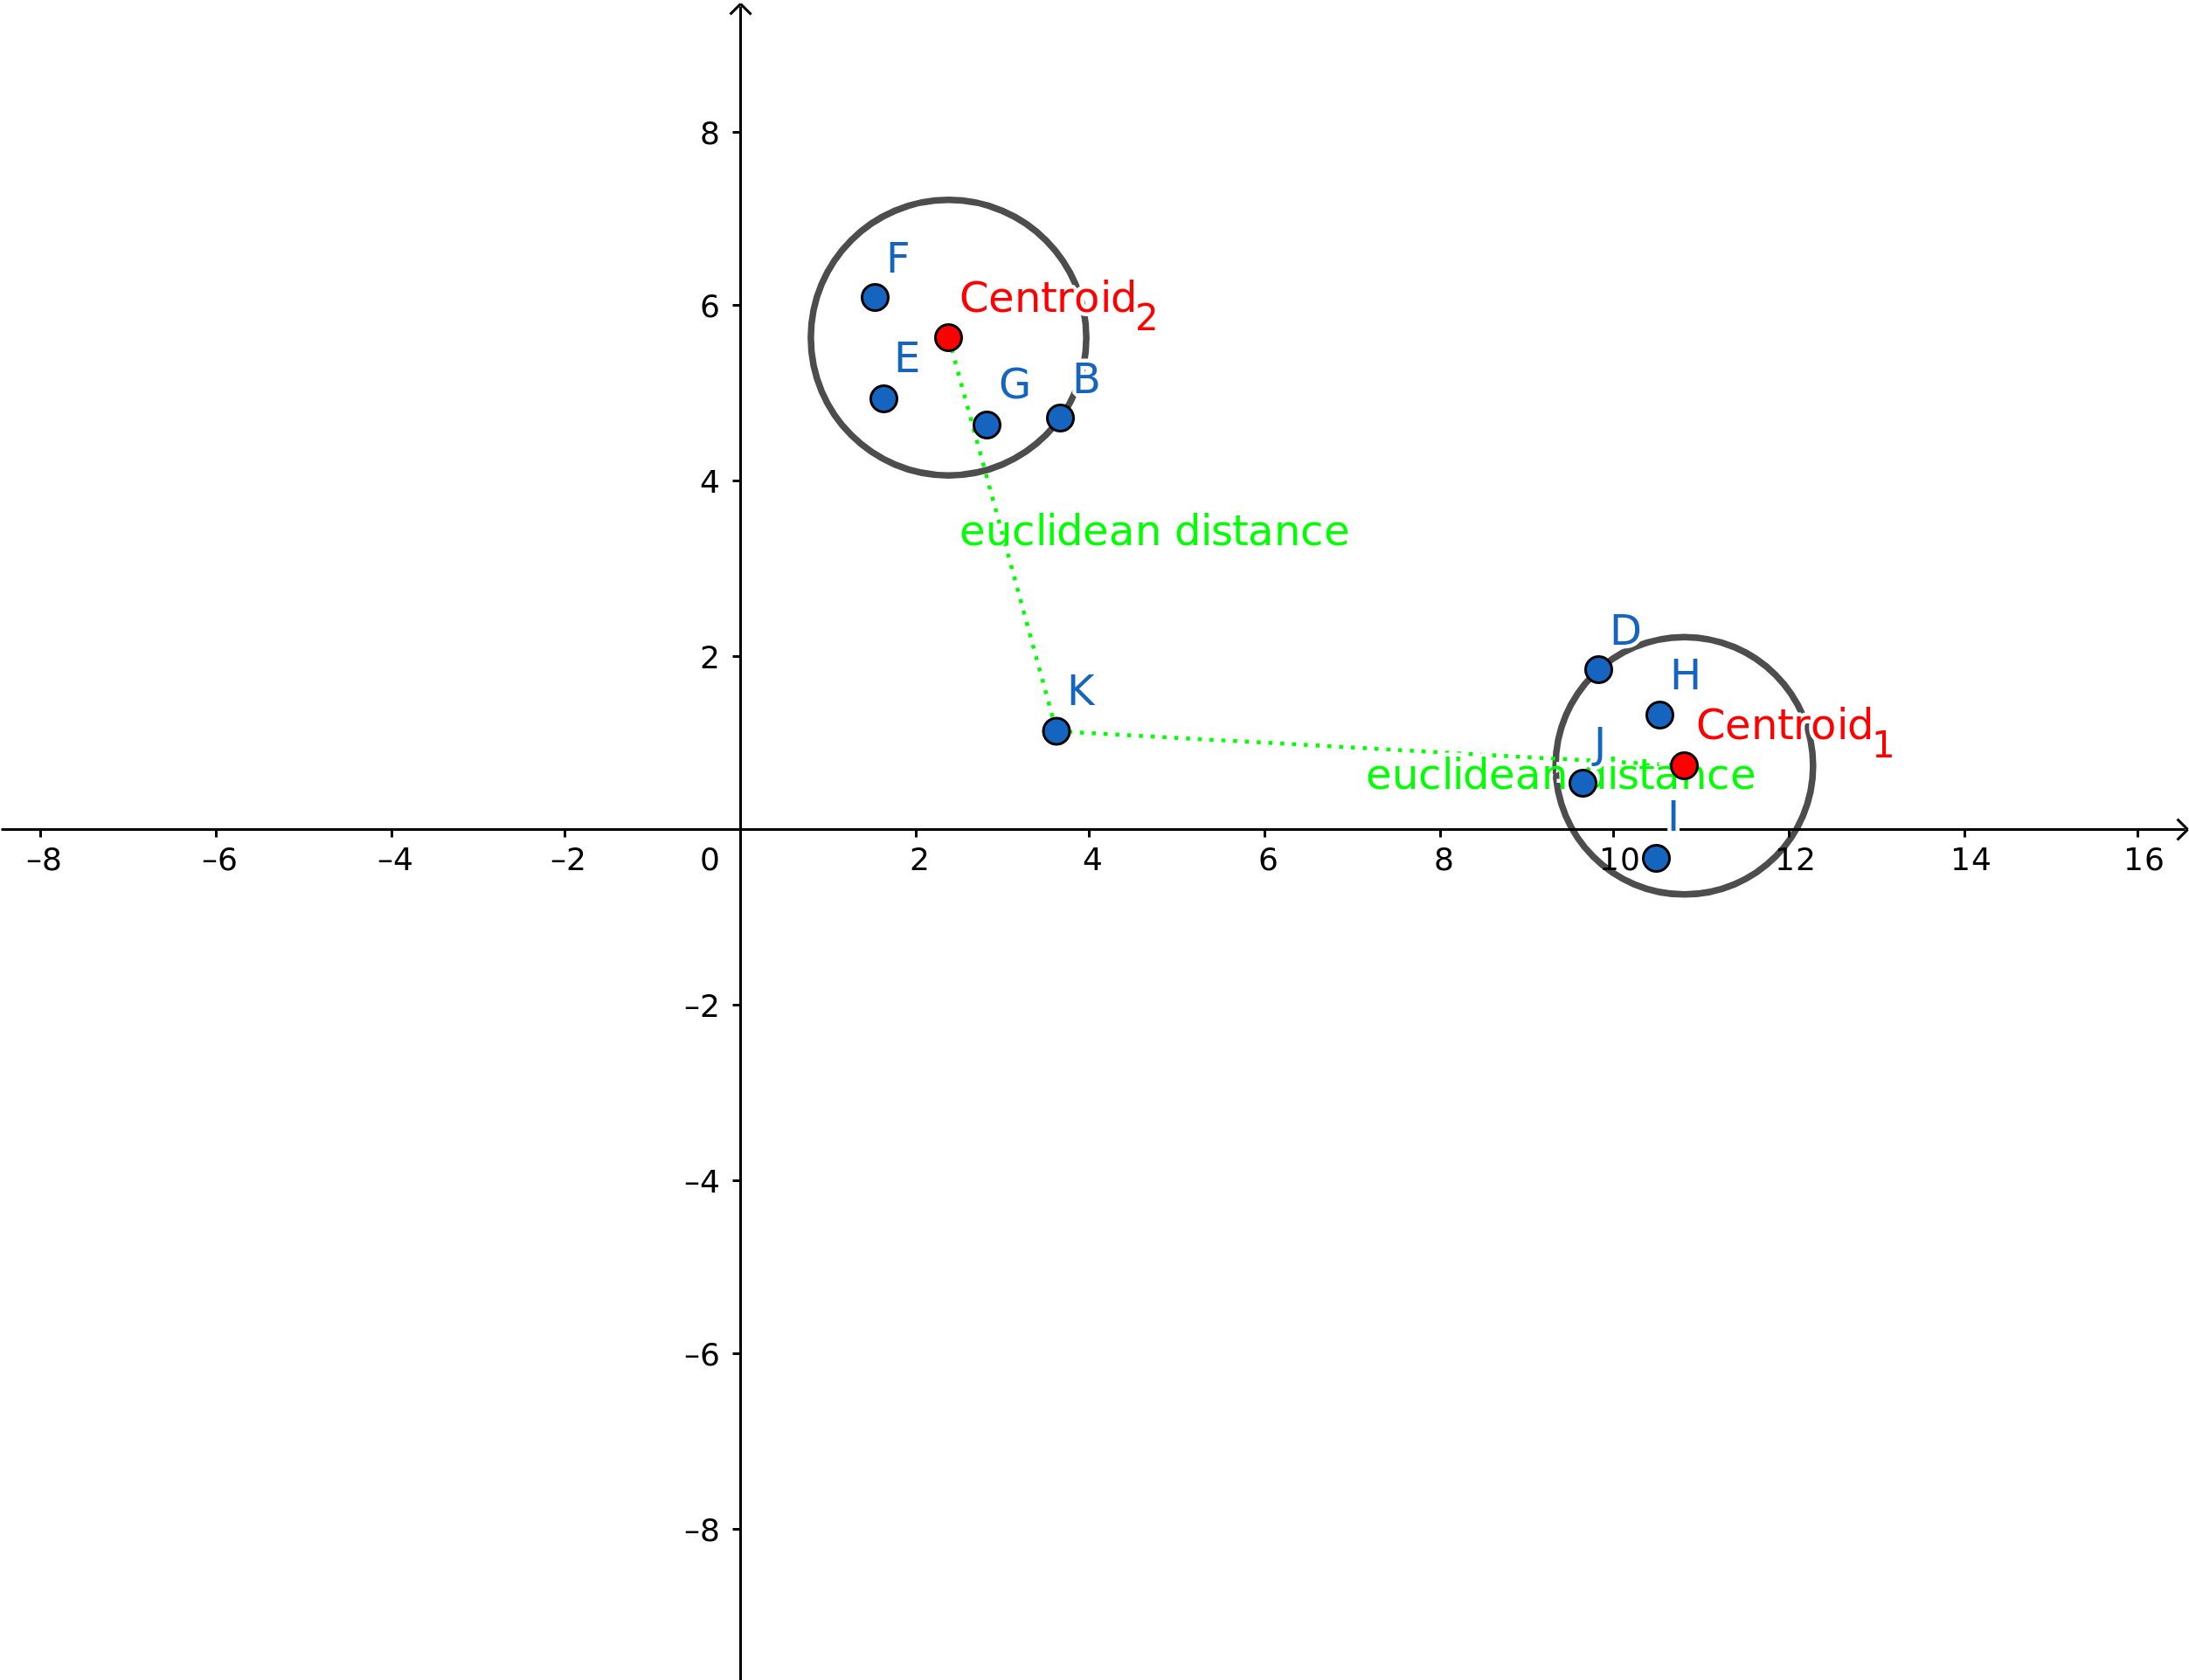
\includegraphics[scale=0.13]{Scoring.png}
  \caption{2D example of Euclidean Distance calculus }
\end{figure}	
		\subsection{Known issues}		
About one mutation out of 15 will fail for undetermined reasons.
			\subsubsection{Context Coherence}
A significant amount of the failing mutations do so because of the mutation transfer mechanism. As said in the dedicated section, this mechanism applies more than one change to the database (potentially the whole database). In specific cases, this property can become problematic. 
More specifically, when the main loop chooses the next mutation and its parent has been the subject of a transfer. In this case, the data embedded in the schemaFuzz data structure may not match the data that are present in the database, this delta may induce a wrong SQL statement that will result in a SQL error (in practice, the DBMS indicates that 0 rows were updated by the statement).
			\subsubsection{Foreign Key constraints}			
For a reason that is not yet clear, some of the implied FKC of the target database can't be properly set to CASCADE mode. This result in a FKC error (mutation fails but the program can carry on)			
			\subsubsection{Tests}
Due to a lack of time and a omission in the project planning, this project's test suit is not yet complete. In its current state, the test suit includes the tests written for the meta data extraction routine as well as a bundle of unit tests that cover the following points :
			\begin{itemize}
			\item{instantiation of the Mutation class}
			\item{Creation of the modification possibilities}
			\item{the do/Undo routine}
			\item{Uniformity of the tree weighting}
			\end{itemize}
			
The following list details the tests that will be implemented in future releases by order of importance.

			\begin{itemize}
			\item{Integration tests}
			\item{Regression tests}
			\item{More complete and specific Unit tests.}
			\item{Performance tests}
			\end{itemize}

			\subsubsection{Code Quality}
The code in its current state is still in beta. This means that the code will be the subject of structural and syntax changes. The following list contains the major aspects of these changes
	
			\begin{itemize}
			\item{Code structure}
			\item{Code concision}
			\item{Code style. More precisely, updating code pieces that cointain bad coding habits}
			\end{itemize}
For example, the following code:
$if(myVariable == 0)$
should be changed to:
$if(0 == myVariable)$
to avoid unwanted affectation in the case of the omission of an $=$ sign. 			
			\clearpage

	\section{Results and examples}
		\subsection{Results on test environment}
The project as been developed primarily to be run against the GNU Taler database. But, a sample database was used throughout the course of the development in order to evaluate the progress of the tool as well as for testing it an environment that would not compromise any real data set.
This sample database contains all the supported types and emulates the structure of a production database.
the following figure shows what the format of output for a standard run is. The tree of mutations is displayed in a text format where each block stands for a successful mutation injection and is delimited by a pair of hooks $[]$. Each block is preceded by a visual representation of the depth in the tree where $--$ indicates one level in the tree. 
The informations provided on each block follow this ordered structure:
		\begin{itemize}
		\item{Mutation ID (ordered)}
		\item{Numerical representation of the Depth in the tree}
		\item{ID of the mutation the modification is attached to}
		\item{The value present in the target field BEFORE the modification}
		\item{The value of the target field AFTER the modification}
		\end{itemize}
				

It is noticeable that the algorithm does not display the tree in depth order but in ID order.
This allows the user to analyze in what order the mutations where injected.

		\bigskip
		\begin{figure} [h!]
			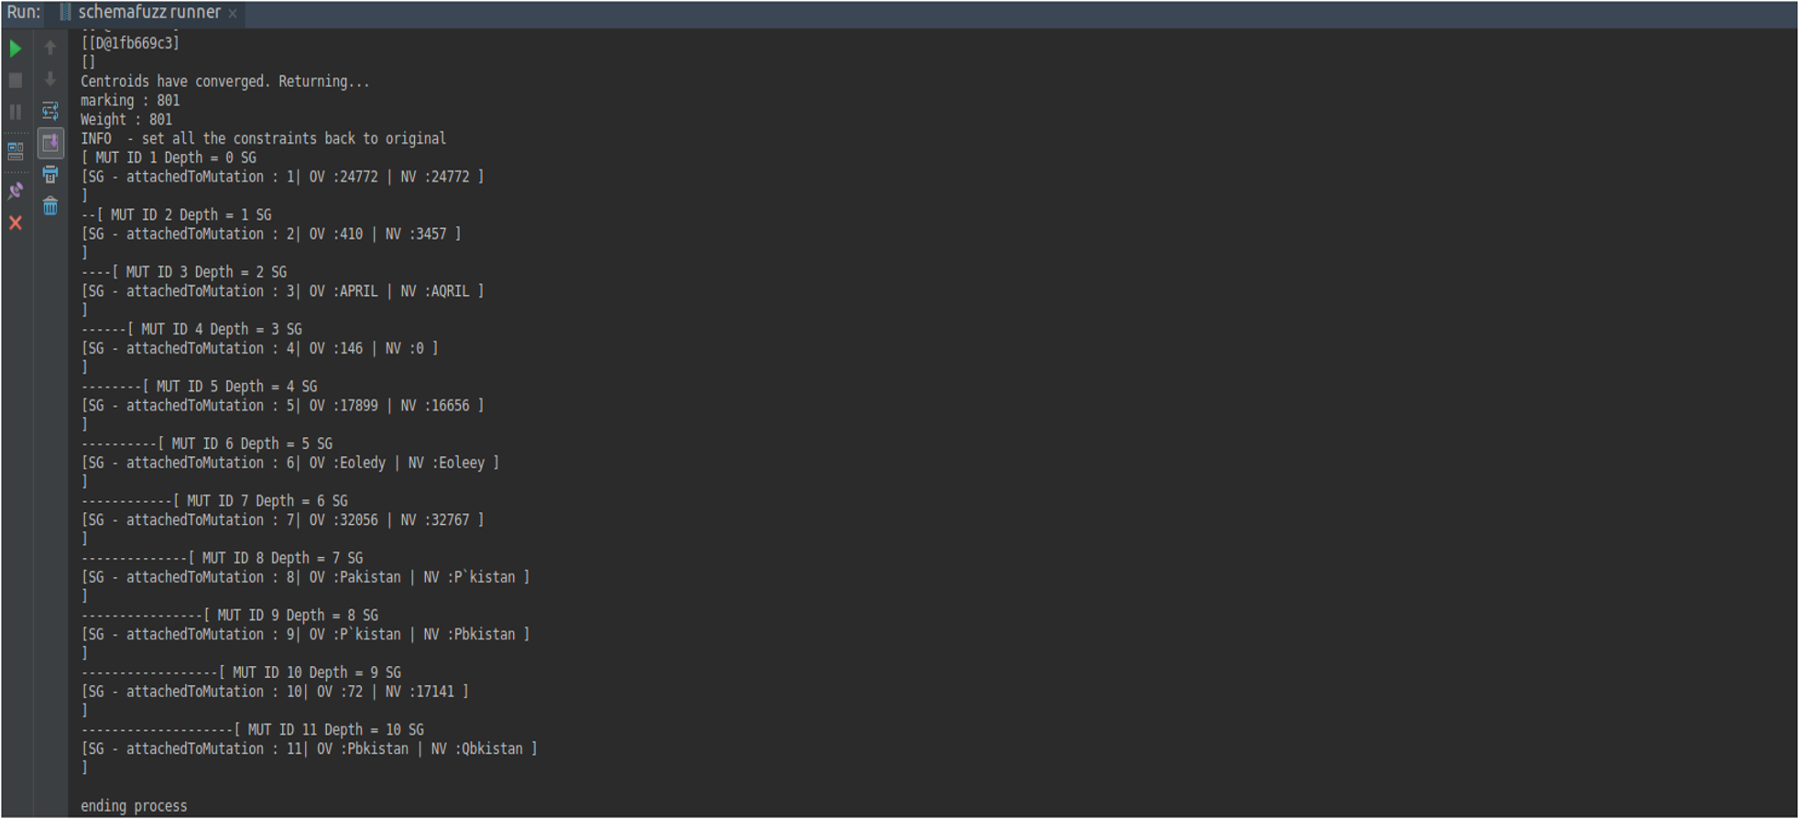
\includegraphics[width=\textwidth]{sc2.png}
			\caption{Example of the output for an execution on the development database}
		\end{figure}
		\bigskip
		
After every successful mutation, the analyzer generates a report that summarizes the response of the target program after the modification was applied.
Every report is structured as follow :

If the program did not crash: report only contains a 0.
	

If the program crashed:
		\begin{itemize}
		\item{"functionNames:" item}
		\item{List representation of the function stack from the crash (ordered from most precise to most general level) }
		\item{"filesNames:" item}
		\item{List representation of the file containing the function call}
		\item{"lineNumbers" item}
		\item{List representation of the line numbers for each function call (the line number of the main function does not appear)}
		\item{"end:" item}
		\item{"path:"item}
		\item{Text representation of the path in the tree from the root. Every line described a previously processed mutation}
		\item{"endpath:"item}
		\end{itemize}
	
		\bigskip
		\begin{figure} [h!]
			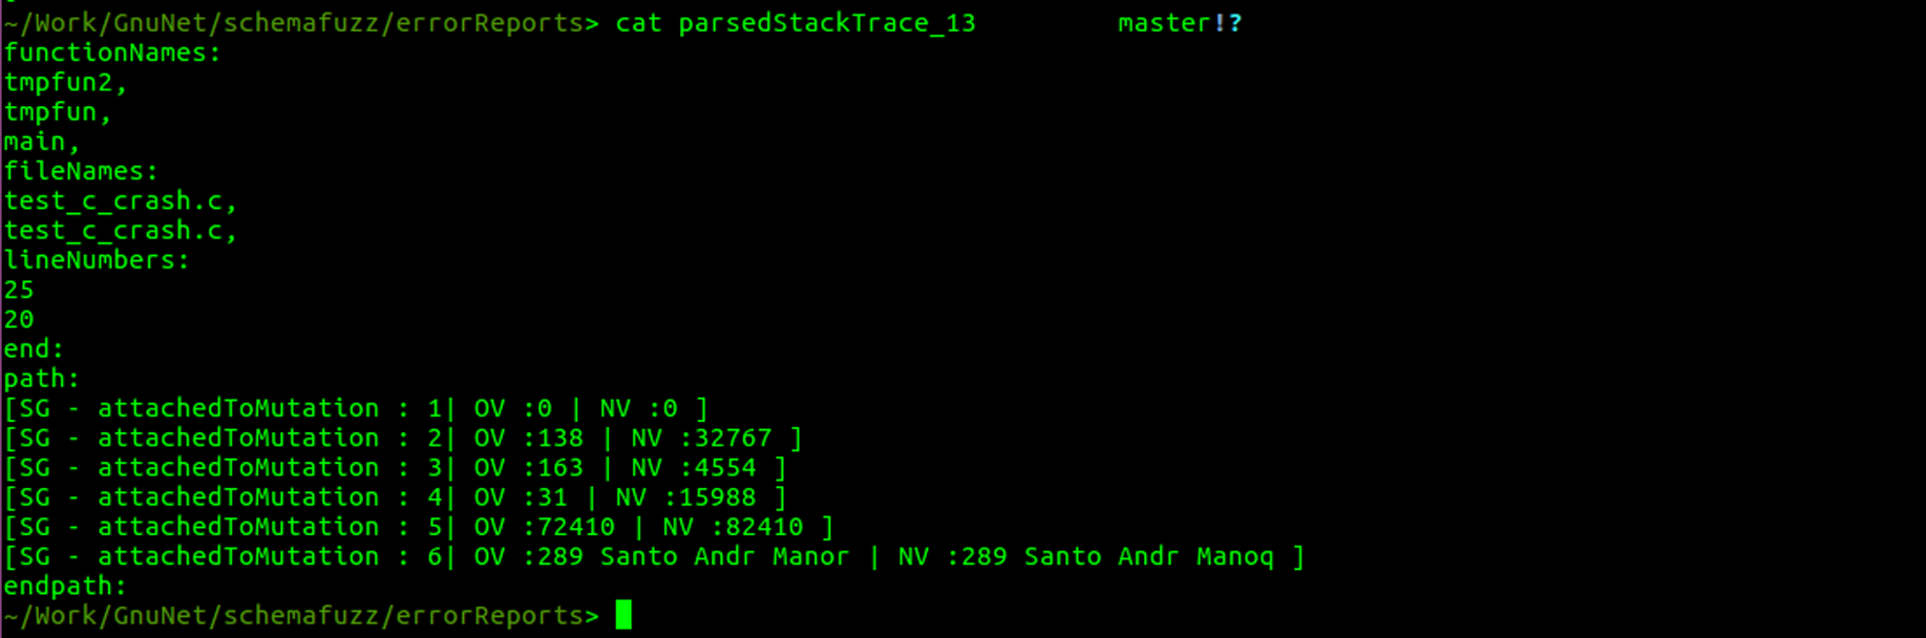
\includegraphics[width=\textwidth]{sc1.png}
			\caption{Example of a generated report for an execution on the development database }
		\end{figure}
		\bigskip
		
		\subsection{Results on the GNU Taler database}

The outcome of the first executions of SchemaFuzz against a sample of the GNU Taler database were promising. The tool itself properly fuzzed the target and the execution ended with a success
code on 9 of the 10 attempts.

\clearpage 		
	
		\bigskip
		\begin{figure} [h!]
			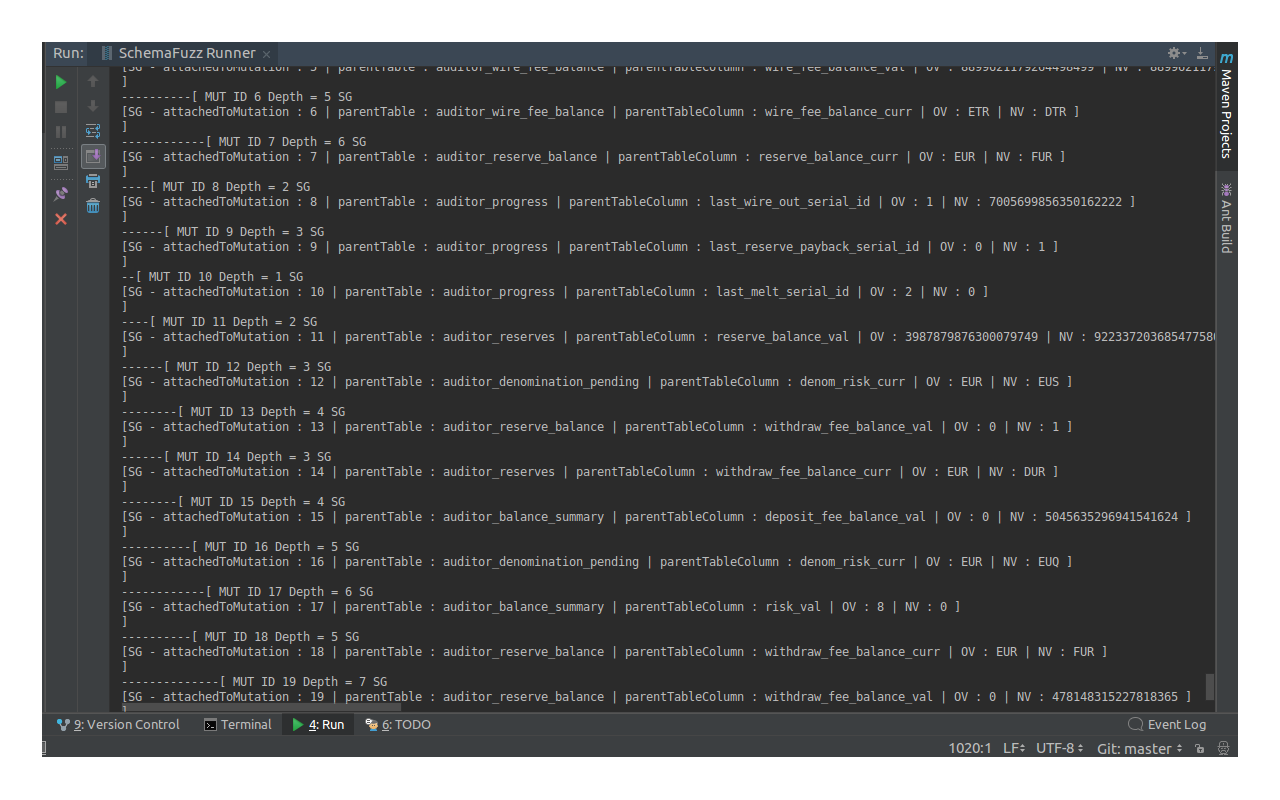
\includegraphics[width=\textwidth]{sc3.png}
			\caption{Example of the output for an execution on a sample of the GNU Taler database}
		\end{figure}
		\bigskip
		
		\paragraph{Vanishing bugs}		
Some of the bugs that were encountered during the test executions were not triggered when running against the GNU Taler database. After comparing the content and structure of both environments, it is likely that this behavior was due to the test database's minimalistic content.
This difference between the outputs when executing the tool on the two different environments helped in debugging some of the code's unexplained behavior. 

For instance, the tool would crash if meeting the following criteria:
	\begin{itemize}
	\item{The last mutation scored better than its parent}
	\item{The last mutation does not have any other modification possibilities}
	\item{In its current state, the tree does not have more than one branch}
	\end{itemize}
	
By running the tool on a more dense database, the bug had vanished. This allowed us to locate the origin of the issue.

		\clearpage
		\bigskip
		\begin{figure} [h!]
			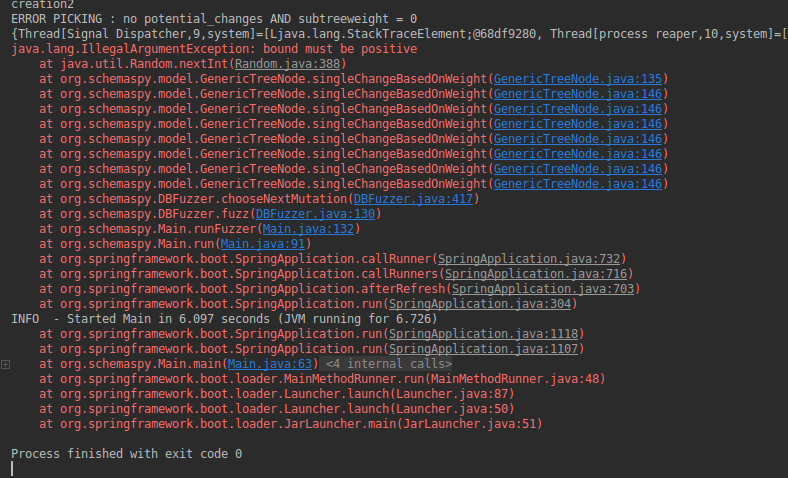
\includegraphics[width=\textwidth]{sc4.png}
			\caption{Example of a bug fixed by changing the environment of execution}
		\end{figure}
		\bigskip
   	       		
	
	\section{Upcoming features and changes}
This section will provide more insights on the future features that might/may/will be implemented as well as the changes in the existing code.

		\subsection{General Report}
In its future state, SchemaFuzz will generate a synthesized report concerning the overall execution of the tool. This general report will primarily contain the most "interesting" mutations (meaning the mutations with the highest score mark) for the whole run. A more advanced version of this report would also take into account other parameters in calculating the ratio for each mutation. By doing so, the analyzer could generate a "global" score that would represent the global value of each mutations.
	
		\subsection{Code coverage}
We are considering changing or simply adding code coverage in the clustering method as a parameters. Not only would this increase the accuracy of the scoring but also give more detail on what the mutation triggered in the target software's code therefore helping locate the origin of the crash. By adding code coverage this tool could make a concrete difference in terms of scoring and informations being generated in the reports between a mutation with a new stack trace in a common code path and a common stack trace in a rarely triggered code path.

		\subsection{Data type Pre-analyzing}
This idea for this feature to be is to implement some kind of "auto learning" mechanism.
To be more precise, this routine is meant to performed a statistical analysis on a representative portion database's content. This analysis would provide the rest of the program the most common values encountered for each field. More generically, this would allow the software to have a global view over the format of the data that the database holds.
Such global understanding of the content format is   interesting to make the modifications possibilities more relevant. Indeed, one of the major limitation of SchemaFuzz is its "blindness".
That is to say that some of the modifications performed in the course the execution of the program are irrelevant due to the lack of information on what is supposed to be stored in this precise field.
For instance, a field that only holds hexadecimal values that go from A01 to A0A even if it has enough bits to encode from 000 to FFF would have a low chance of triggering a crash if this software modifies its value from A01 to A02.
on the other end, if the software modifies this same field from A01 to B01, then a crash is much more likely to be discovered.
Same principle applies to strings. Suppose a field can encode 10 characters.
the pre-analysis, detected that, for this field, most of the value were surnames beginning with the letter  “a". Changing this field from  “Sylvain" to  “Sylvaim" will probably not be effective. However, changing this same field from  “Sylvain" to  “NULL" might indeed trigger an unexpected behavior. 
  
This pre-analysis routine would only be executed once at the start of the execution, right after the meta data extraction. The result of this analysis will be held by a specific object. 
this object's lifespan is equal to the duration of the main loop's execution. That way, every mutation can benefits from the analysis data.
		
		\subsection{Centralized anonymous user data}
SchemaFuzz's efficiency is tightly linked to the quality of its heuristics. This term includes the following points 
		\begin{itemize}
		\item{Quality of the possible modifications for a single field}
		\item{Quality of the possible modifications for each data type}
		\item{Quantity of possible modifications for a single field}
		\item{Quantity of supported data types}
		\end{itemize}
Knowing this, we are also considering for futures enhancements an anonymous data collection  for each execution of this tool that will be statistically computed to determine the best modification in average. This would improve the choosing mechanism by balancing the weights  depending on the modification's average quality. Modifications with higher average quality would see their weight increased (meaning they would get picked more frequently) and vice versa. 			



	\section{Contributing}
You can send your ideas and patch proposals at \url{erwan.ulrich@gmail.com} \\*

\appendix	
\newpage

\section{Internship organisation} 
	\subsection{Introduction}

This section is meant to be added to the University version of this documentation. It will be written as Erwan Ulrich and will focus on the different aspects of the organization of the project. The following text will also be written with a more personal and more critical point of view as a mean of self analyze.

	\subsection{Calendars}
	
The	SchemaFuzz project has had since its genesis a quiet clear view of how the development should evolve. The desired features have been discussed and the big picture had been designed to fit the time that the main developer had for his work at this position.
The project had to pass trough different phases of development that are detailed in the following time line diagram. %% insert timeline diagram here.

Some of the tasks of the above time line were completed on time, some others were delivered late, and some were delayed in the time line because of the previous point.
In the end, the project was lead in a way that is best described by the following time line diagram.    %% insert timeline diagram here.

Those two diagrams differ on some points. This is one of the major failures for the development of this project throughout the course of these 6 months. 
There are several reasons that explain why this project could have been lead in a better way.
they will be detailed and discussed in the next section. 

	\subsection{Organizational failures}
This section has a particular value in this report, it is on the first hand a description of why the SchemaFuzz did not meet all of its defined goals.
Other the other hand, it is a personal reminder of what should be improved in my work habits and general organization when leading a project of such a large size. 
	
	\begin{itemize}
	\item{Defining tasks/features as daily/weekly sub goals}
	\item{Improving multitasking} %% bad title.
	\item{Setting up more fluid communication}
	\end{itemize}		

	\subsection{Positive outcomes}
Throughout the development of the project, I have had the chance to acquire many new capacities and improve many of my own skills. I will give more insights on what this project and, more generically, what this internship as a developer for a GNU package, has brought me.

		\subsubsection{Technical aspect}
		
		\paragraph{Java language}
In many ways, this project has been a real challenge. But the main difficulty that I encountered was the technical challenge that rose up when the project started. Indeed, it was my first time conducting a project of the size of SchemaFuzz. The size of the project and the fact that I was the only one developing the tool implied that every aspect of the project, independently of the language that was used for each module, had to be imagined and implemented with my two hands.
Even if I was already accustomed to Java programming, I got struck by the complexity and the architecture of a "real" in-production software like SchemaSpy which I had to look into to get the meta data extraction routine.
This was my first improvement. Code structure. Even if my coding capacities can still be perfected in many ways, I feel like understanding/re-using complex and well structured code gave me a much better idea of what "good code" really is. Integrating these concepts empowered my development skills and I am now much more confident about it.

Apart from the Java language, which I was already familiar with, I also had the chance to get my hands of new technologies (or technologies I never really had the chance to practice in real conditions). 

			\paragraph{SQL language}
SchemaFuzz is a database fuzzer. Naturally, A major component of the work for its development was to create and handle SQL requests and responses. In order to do that, I had to document myself for a while as I was lacking some knowledge on databases in general. After gaining a better understanding of how databases operate theoretically, I had to go into more depth concerning the inner structure of constraints and the way data types are encoded for most DMBS.
This brings me to my next point regarding the handling of SQL in this project.

			\paragraph{DBMS(PostgreSQL)} 
SchemaFuzz's first and foremost import goal is to help in the debugging and maintenance of the GNU Taler payment system. GNU Taler databases are managed by the PostgreSQL DBMS. Therefore, the natural choice of technology for SQL management in this project was obvious.
Not having ever worked with PostgreSQL before, I had to adapt my habits when dealing with the DBMS itself.
By doing so, and stumbling on error messages I had never seen before, I had the chance to get into more depth in the structure of DBMSes in general. In particular, I had to get my hands on the inner PostgreSQL tables in order to understand how different databases were managed within the same environmental.

			\paragraph{Shell/Bash Scripting} 
As a part of the development of the analyzer for SchemaFuzz, I have had the chance to build up several bash scripts. This  was to me a true pleasure as well as very instructive.
Spending some time on writing parsing script had me look into how parsing is usually implemented for such jobs.
Having this experience with me, I now better understand how each and every component of a same project connects to each other. 
Even though I was aware of the power of scripting in general, I have now come to understand how much of a crucial skill it is to understand and be able to write scripts when working in a Linux environment.
In the big picture, I feel like I have earned a precious asset by practicing scripting on a technical level. This also gave me the chance to develop my own script in the frame of personal use in my own environmental. Going through more conceptual and theoretical documents on what scripting really is and how it should be used.
   			
			 \paragraph{LateX}
By writing this documentation, I had to learn how to create and process properly presented and properly styled scientific documents. In this process, I have first learned and then practiced LateX as well as the very handy Tikz and metaUML packages used for graphical representations.
Creating and implementing (in this case) graphics I did not consider to be a real coding challenge, but some of them proved me terribly wrong. Spending time on finding the right syntax for what I wanted to show strengthened my project management skills and comforted me in the belief that presentation and creation of a project are two sides if the same coin and that both should be treated with the same amount of seriousness.  			  
	

		\subsubsection{Human aspect}
		
			\paragraph{Languages}
The development of my project was conducted in German-speaking environment, which is a language I am not very familiar with. 
This lead to having any kind of communication both regarding the project and other subjects in English. This participated in my improvement in both oral and written English (this document is also an excellent training for written content) as well as my overall comprehension.
Apart from the pure linguistic point of view, discussing complex topics in English gave me the keys to expressing ideas and concept in a more concise and clearer way. 			

			\paragraph{Political maturity}
Disclaimer. With this paragraph, I am not pushing forward any idea in particular, all I intend to do is explain with more detail and insights on how rich the environment was during this internship.			
			
Surprisingly, I have had the chance to meet many people that shared various political points of view regarding computer science and technologies. In these subjects it was a truly enriching process to debate things such as morality, ethic or freedom.
Some other topics that are further away from science were brought up such as vegan-ism, green energies, or anarchism.
I hold very dearly the moments I shared speaking and confronting my own ideas because I feel like this has allowed me to gain maturity in my political positions.		
	
	\clearpage

	\subsection{Conclusion}
   
The development of SchemaFuzz and my work for GNU Taler was spread out on a 6 months duration.
Within this time lapse, I have discovered the fields of research and real software development.
This discovery has been very beneficial to me in the sens that it gave me the chance to acquire experience both on the theoretical and technical sides as well as mastering some new technologies and new aspects in the field of computer science in general.

My work for GNU Taler was primarily to imagine,conceptualize and develop a database oriented fuzzing tool. 
First, I focused on bringing the software from a shape of "general idea" that was given to me by my internship supervisor to a concrete and structured project. In the process of creation, I started with defining what precise features were critical and with what technology they would be implemented.

The main task of SchemaFuzz is to inject malformed data into a specific database in order to trigger crashes or unexpected behavior from the program that uses the content of this database.
By working on this project for the past 6 months, I have brought it to a point where it fulfills its main task. I have uses a sample database contain content with a wide variety in terms of data types to test the project all along the course of the development. However, the application is meant to evolve to a more advanced state. Such a big project requires much more time than what I had to be fully operational.

Finally, I am convinced that the realization of this project was a truly rewarding experience on all academical, technical and human aspects. All the knowledge acquired as GNU developer strengthened the concepts I had learned in my academical courses. Moreover, this internship is an excellent social experience thanks to the amount of contact with very bright professors, PhD students and other interns.     
   

	
	\bibliography{testcite}		
			
\end{empfile}
\end{document} 
